\chapter{VRPTW via AI}
In this chapter, we will review the current end-to-end \gls{ai} methods for solving \gls{vrp} and propose our extension for solving \gls{vrptw}.

Machine learning and artificial intelligence have been replacing many hand-engineered algorithms and providing state-of-the-art results. In recent years, reinforcement learning \ref{rl} and advances in attention models \ref{attention} has shown great promise to disrupt the field of heuristics algorithms \cite{rl-constraint-opt, attention-route, dpdp}. Heuristics algorithms \cite{heuristics-algo} are incomplete methods that can compute solutions efficiently, but are not able to prove the optimality of a solution. Most of the business challenges do not require the most optimal exact solution \cite{excat-algo} but focus on approximation of the optimal solution in a reasonable time.

\section{Related Work}
Researchers have been mainly active in solving general \gls{vrp}...
TODO

\section{Solution}
The end-to-end \gls{ai} method pro solving \gls{vrptw} is extension of the work done by Kool et al. \cite{attention-route}. 

Let us describe the high-level concept behind the method. Consider we have a model as blackbox which takes \gls{vrptw} instance as an input and outputs probabilities for all the \gls{vrptw} nodes. The probability represents which node should be visited next and by following to the most probable node we get a partial solution which will be considered by the blackbox. We iterate this process until all nodes have been visited and we acquire a feasible plan as shown on Figure \ref{fig:attention-route-diagram}.

    \begin{figure}[ht]
        \centering
        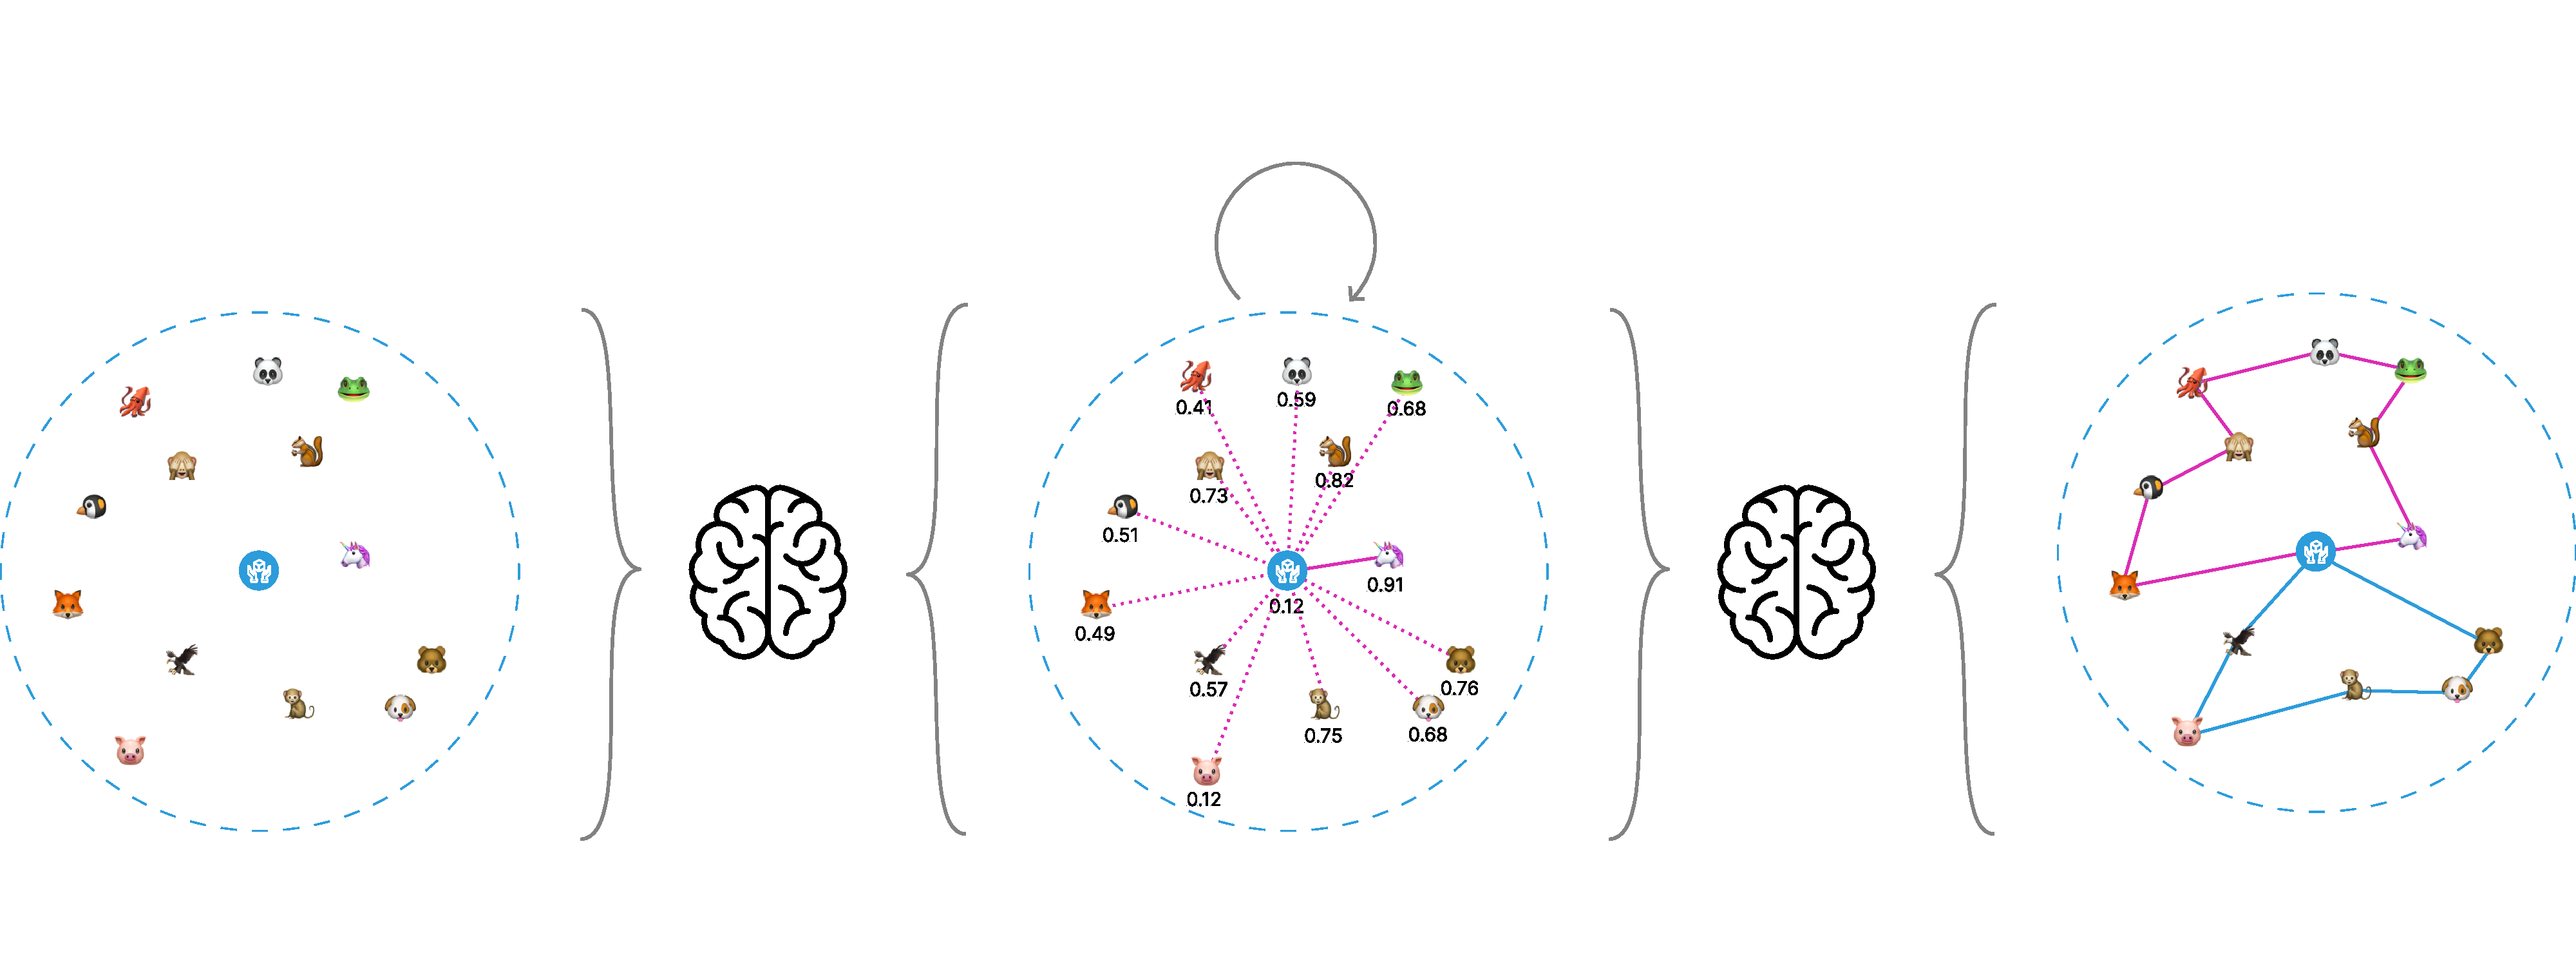
\includegraphics[width=1.0\textwidth]{resources/vrptw-ai/attention-route-diagram.pdf}
        \caption{High-level concept behind the used method.}
        \label{fig:attention-route-diagram}
    \end{figure}

    \subsection{Model Architecture}
    The model architecture \cite{attention-route} leveraging recent advancements in attention mechanism is here extended by the time window constraint. The model is built upon transformers \ref{transformer}, graph attention network \ref{graph-attention-network}, and reinforcement learning \ref{rl}. The network structure is encoder-decoder that fits well for solving sequential decision problems. The structural input instance is extracted by the encoder \ref{vrptw-encoder} and then the solution is incrementally constructed by the decoder \ref{vrptw-decoder}.
    
    The \gls{vrptw} input instance is consisted from:
    \begin{itemize}\label{input-data}
        \item $X = \{x_1, \cdots, x_n\}$ where $x_i$ is two-dimensional coordinates in the euclidean space.
        \item $x_0$ is the location of depot.
        \item $D = \{d_1, \cdots, d_n\})$ is the demand capacity for each of the locations.
        \item $T = \{(e_1, l_1), \cdots, (e_n, l_n)\})$ is time windows for each of the location where $e_i$ is the beginning and $l_i$ is the end of the considered time window.
    \end{itemize}
    
    The output is the solution of VRPTW instance and is represented as a permutation $\pi$ of locations $X \cup x_0$.
    \begin{itemize}
        \item $\pi = \{\pi_1, \cdots, \pi_T\} \in \{x_0, \cdots, x_n\})$ 
    \end{itemize}
    
    \subsubsection{Encoder}\label{vrptw-encoder}
    The encoder uses graph attention network \ref{graph-attention-network} to embed the node features to graph embedding. Then the decoder architecture is the same as the decoder of transformer \ref{transformer}. Typicaly, the decoder of transformer uses positional encoding \cite{positional-encoding} to embed the input, but in this case it has been replace with \gls{gat} \ref{graph-attention-network} since we deal with graph-based structure and the input order does not matter.
    
    The first step is to perform the initial embedding of input data \ref{input-data} via learned linear projections as in \gls{gat}. The $h_{i}^{l}$ represents the node embedding of layer $l \in \{0, \cdots, N\}$ (N=3).
    \begin{equation}
        \widetilde{x} = \text{concat}(X, D, T)
    \end{equation}
    \begin{equation}
        h_{i}^{0} = \begin{cases} W \widetilde{x}_i + b_i &\mbox{if } i > 0 \\ W \widetilde{x}_0 + b_0 & \mbox{if } n = 0 \end{cases}
    \end{equation}
    
    The node embeddings are updated via $N$ attention layers, each containing multi-head attention \ref{multi-head-attention} (M=8) and a fully connected feed-forward network with normalization. The structure is identical to transformer's encoder \ref{transformer} with additional support of graph structure \ref{graph-attention-network} as shown on Figure \ref{fig:encoder-diagram}.
    
    \begin{figure}[ht]
        \centering
        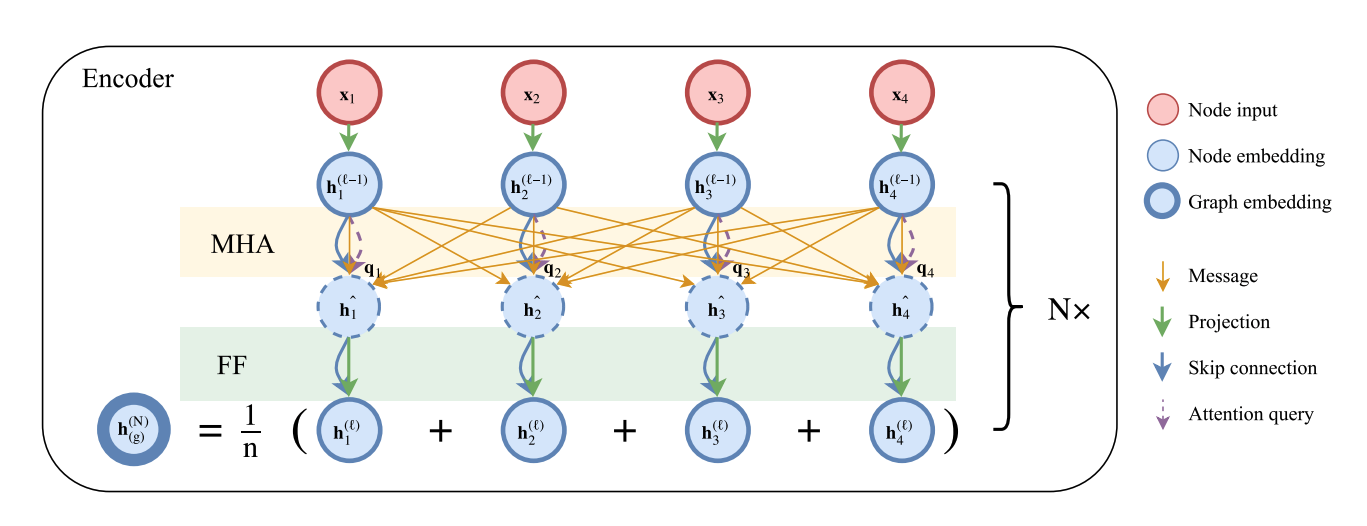
\includegraphics[width=1.0\textwidth]{resources/vrptw-ai/encoder-diagram.png}
        \caption{Encoder layers \cite{attention-route}}
        \label{fig:encoder-diagram}
    \end{figure}
    
    The equation \ref{encoder-qkv} calculates the query $Q$, key $K$ and value $V$ of multi-head attention layer using the node embeddings and weights $W_m^Q$, $W_m^Q$, and $W_m^Q$, respectively. The number of heads is represented by $m \in \{1, \cdots, M\}$ (M=8).
    
    \begin{equation}\label{encoder-qkv}
        \textbf{q}_{im}^l = W_m^Q h_i^(l-1), \textbf{k}_{im}^l = W_m^K h_i^(l-1), \textbf{v}_{im}^l = W_m^V h_i^(l-1)
    \end{equation}
    
    The query and key values are used in calculating the compatibility $u_{ijm}^l$ of node $i$ with a node $j$ \ref{mha-compatibility}. If node $i$ is not adjecnt to node $j$ then they are not compatible and the value is set to a large negative number.
    
    \begin{equation}\label{mha-compatibility}
        u_{ijm}^l = \begin{cases} q_{im}^l k_{jm}^l &\mbox{if $i$ adjacent to $j$} \\ -\infty &\mbox{otherwise} \end{cases}
    \end{equation}
    
    The attention score $a_{ijm}^l \in [0,1]$ is calculated using softmax from the compatibility values of nodes \ref{encoder-attention-score}
    
    \begin{equation}\label{encoder-attention-score}
        a_{ijm}^l = \dfrac{e^{u_{ijm}^l}}{\sum_{j'=0}^n e^{u_{ij'm}^l}}
    \end{equation}
    
    The transformed $h'_{im}^l$ \ref{h-prime} aggregates all attention scores across neighbour nodes, which is based on GAT \ref{graph-attention-network}. 

    \begin{equation}\label{h-prime}
        h'_{im}^l = \sum_{j=0}^n a_{ijm}^l v_{jm}^l
    \end{equation}
    
    Finally, we may calculate the multi-head attention \ref{transformer} for layer $l$ as a function of $\{h_1^{l-1}, \cdots, h_n^{l-1}\}$ through $h'_{im}^l$.
    
    \begin{equation}
        \text{MHA}_i^l(h_1^{l-1}, \cdots, h_n^{l-1}) = \sum_{m=1}^M W_{m}^O h'_{im}^l
    \end{equation}
    
    \begin{equation}
        \widetilde{h}_i = \text{BN}^l(h_i^{l-1} + \text{MHA}_i^l(h_1^{l-1}, \cdots, h_n^{l-1})))
    \end{equation}    
    \begin{equation}
        h_i^l = \text{BN}^l(\widetilde{h}_i + \text{FF}^l(\widetilde{h}_i))
    \end{equation}
    
    In the final layer, the encoder computes the aggregated embedding of the input graph as the mean of the final node embeddings.
    \begin{equation}
        h^N = \dfrac{1}{n} \sum_{i=1}^m h_i^N
    \end{equation}
    
    The output of the encoder's final layer is passed to the decoder, which is detailed in the next sections \ref{vrptw-decoder}.
    
    \subsubsection{Decoder}\label{vrptw-decoder}
    Decoder works sequentially through timestamps $t \in \{0, \cdots, n\}$, at each timestamp one node is selected to be visited based on partial route $\pi_{1:t-1}$. It is predicting the probability distribution over nodes according to the node embedding and context vector of the encoder \ref{vrptw-encoder}.
    
    The decoder uses a new context vector $h_{c}^{'}$ which represents the state \ref{rl} and it goes as follows:
    \begin{equation}\label{decode-state-vec}
        h_{c}^{'} = \begin{cases} \text{concat}(h_N; h_0^N; D_t) & \mbox{if } t = 0 \\ \text{concat}(h_N; h_{\pi_{1:t-1}}^N; D_t) & \mbox{if } t > 0 \end{cases}
    \end{equation}
    The state of $h_{c}^{'}$ is concatenation of $h_N$, the output of the encoder, $h_{\pi_{1:t-1}}^N$, the embedding of previous partial solution, and $D_t$, the remaining demand capacity of the vehicle.
    
    Since the decoder architecture is transformer \ref{transformer} a multi-head attention layers continue and the are resposible for chosing the next node to visite which is defined as an action \ref{rl}.
    
    TODO MHA context embedings + mask with compatibility
    TODO The calculation of compability+ mask with compatibility
    
    The final layer calculates the desired probability $p_{\theta}('pi_t|X, \pi_{1:t-1})$, a logit layer. It is predicted with a single-head attention layer as follows:
    
    \begin{equation}
        q = W^Q h_c, k_j = W^K h_j^N
    \end{equation}
    
    \begin{equation}
        u_j = \begin{cases} C . \text{tanh}(q^T k_{c}) &\mbox{if }  d_j <= D_t \text{ and } x_j \notin \pi_{1:t-1} \\ -\infty &\mbox{otherwise} \end{cases}
    \end{equation}
    
    If we would consider time window as a hard contraint, the calculation of compatibility would have to extended with condition to check fesibility of time windows.
  
    \begin{equation}\label{encoder-attention-score}
        p_{\theta}('pi_t|X, \pi_{1:t-1}) = \dfrac{e^{u_j}}{\sum_{j'=0}^n e^{u_j'}}
    \end{equation}
    
    \begin{figure}[ht]
        \centering
        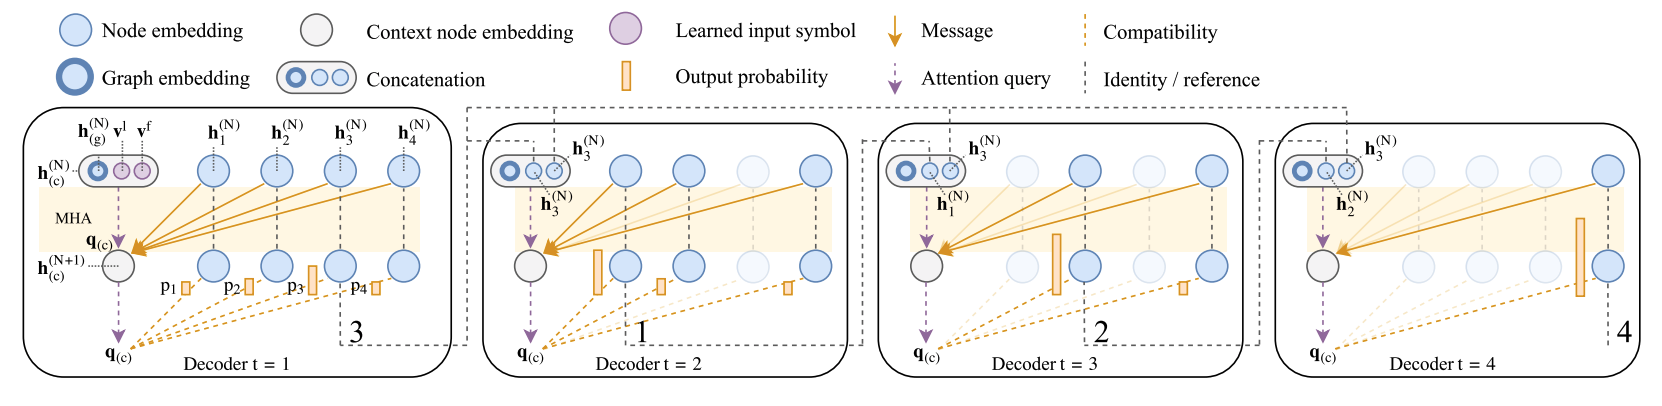
\includegraphics[width=1.0\textwidth]{resources/vrptw-ai/decoder-diagram.png}
        \caption{TODO \cite{attention-route}}
        \label{fig:encoder-diagram}
    \end{figure}
    
    \subsection{Reinforcement Learning}\label{vrptw-rl}
        
    \subsection{Integrating Distance Matrix}
    Multidimensional scaling
